%%%%%%%%%%%%%%%%%%%%%%%%%%%%%%%%%%%%%%%%%%%%%%%%%%%%%%%%%%%%%%%%%%%%%%%%%%%%%%%%
% ScaleNav -- ICRA-style manuscript draft (v2, restructured)
% Compile with ./build.sh
%%%%%%%%%%%%%%%%%%%%%%%%%%%%%%%%%%%%%%%%%%%%%%%%%%%%%%%%%%%%%%%%%%%%%%%%%%%%%%%%

\documentclass[letterpaper,10pt,conference]{ieeeconf}
\IEEEoverridecommandlockouts
\overrideIEEEmargins

\usepackage{amsmath}
\usepackage{amssymb}
\usepackage{booktabs}
\usepackage{graphicx}
\usepackage{xcolor}
\usepackage{placeins}

\newcommand{\vect}[1]{\boldsymbol{#1}}
\newcommand{\mat}[1]{\mathbf{#1}}
\newcommand{\R}{\mathbb{R}}
\newcommand{\blank}{--}

\title{\LARGE \bf
ScaleNav: Semantic Foresight on Persistent Free-Space Graphs\\
for Vision-Based Aerial Navigation
}

\author{First Author$^{1}$ and Second Author$^{2}$%
\thanks{This work was not supported by any organization.}%
\thanks{$^{1}$First Author is with the Affiliation,
        {\tt\small first.author@example.com}}%
\thanks{$^{2}$Second Author is with the Affiliation,
        {\tt\small second.author@example.com}}%
}

\IEEEaftertitletext{%
  \begin{center}
  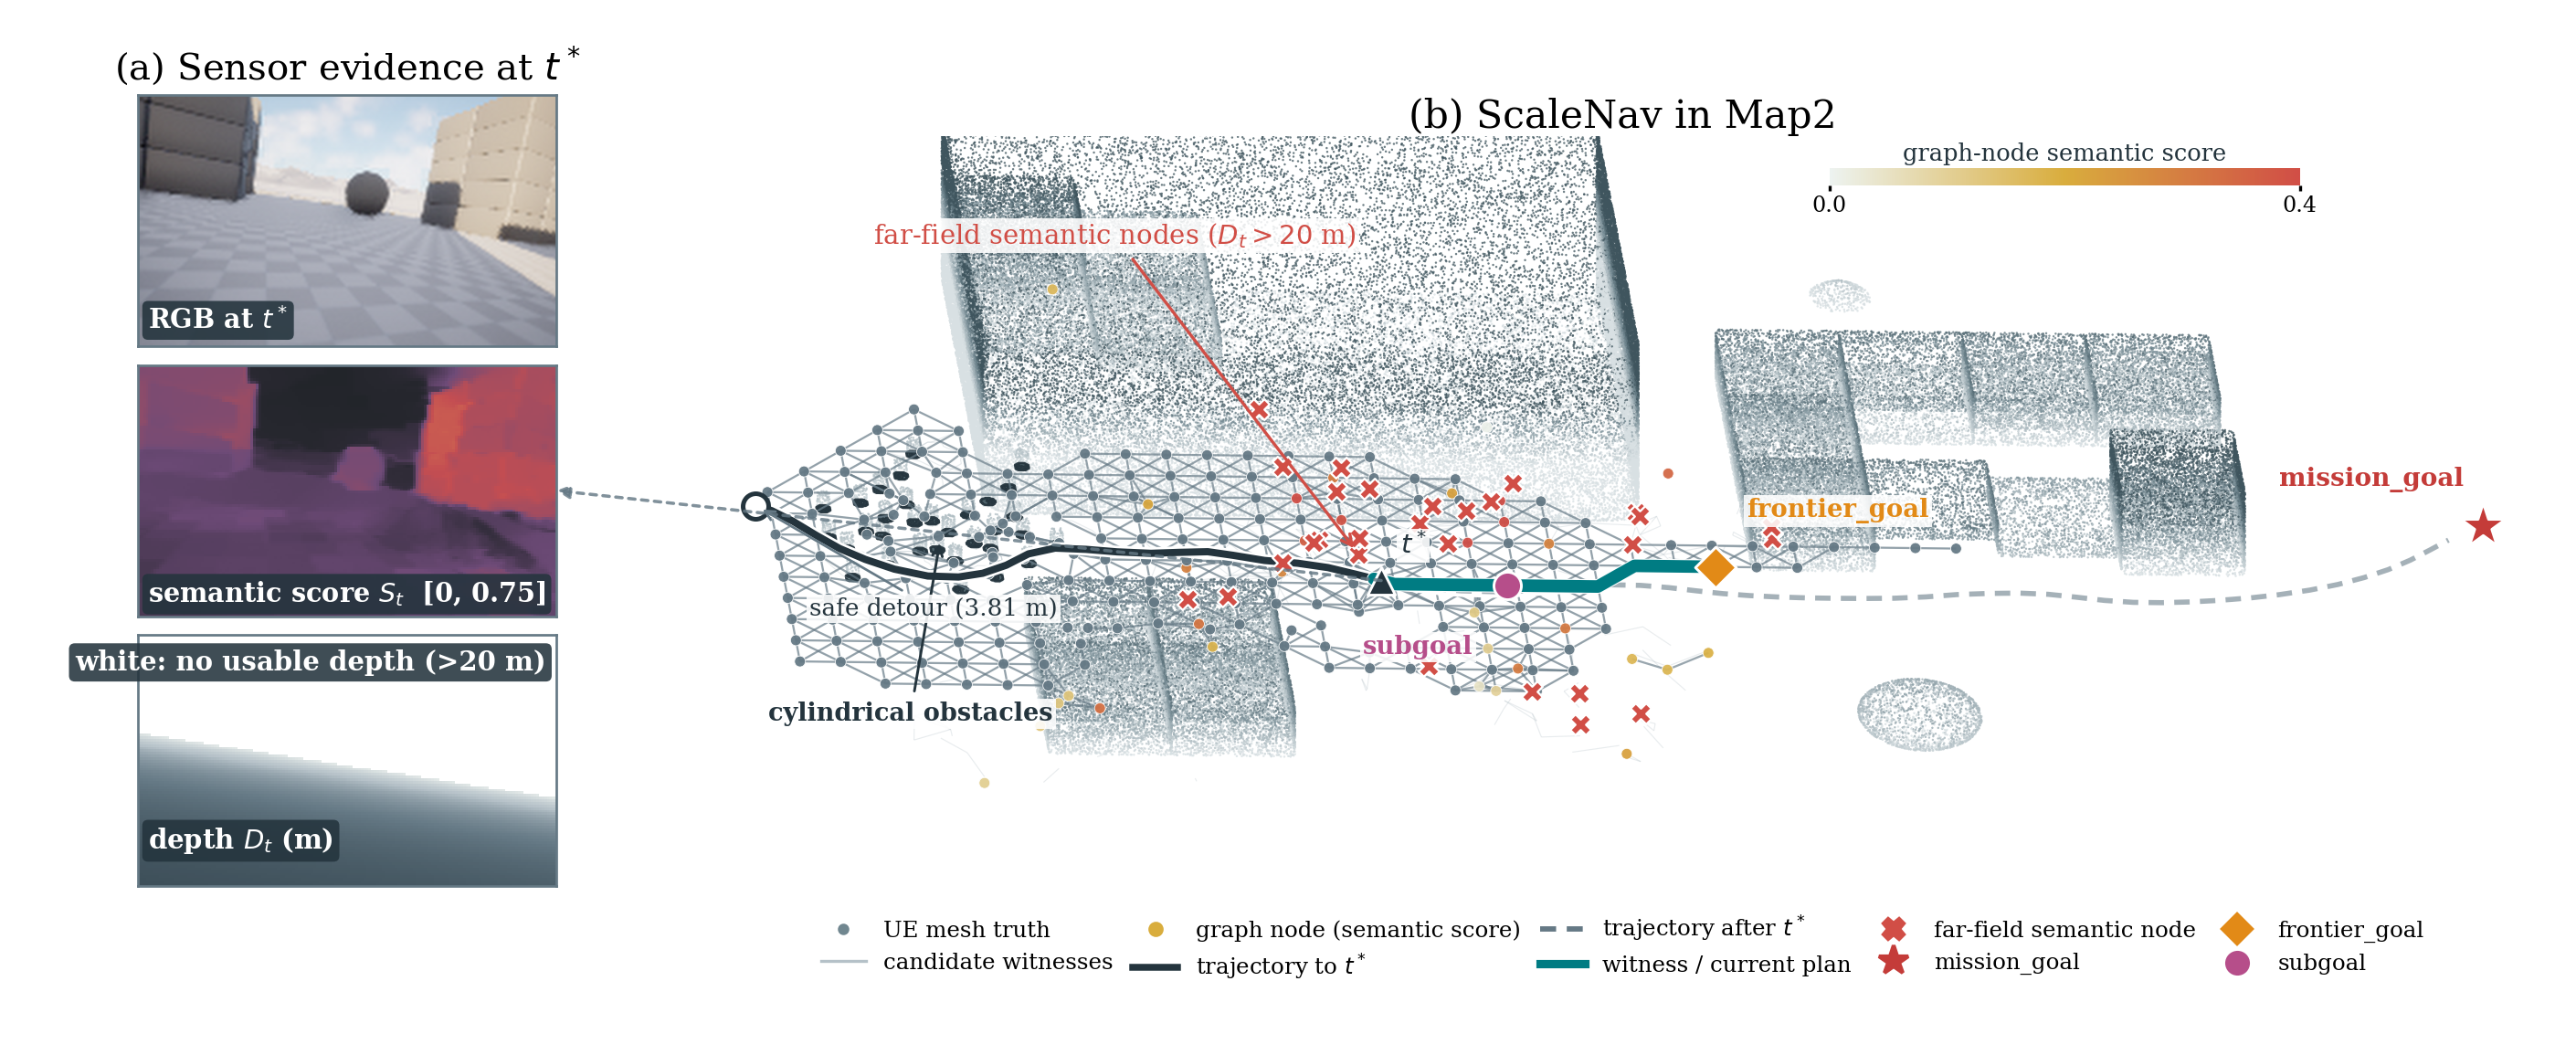
\includegraphics[width=0.98\textwidth]{pics/teaser.pdf}
  \vspace{3pt}
  \parbox{0.98\textwidth}{\footnotesize
  \textbf{Fig. 1.}~ScaleNav flying in Map2 at time $t^*$.
  (a)~RGB, semantic score, and depth at $t^*$. Depth has no valid return
  beyond $20$~m, while the semantic heatmap still responds to the distant
  structure.
  (b)~Top view of the mission over the UE mesh. Node color encodes semantic
  score. Crosses mark far-field semantic nodes within the influence radius of
  this graph slice. The slice spans $\pm2$~m around the navigation height.
  Graph and path states are logged within $90$~ms of $t^*$.
  \texttt{mission\_goal}, \texttt{frontier\_goal}, and \texttt{local\_goal}
  denote the task, route, and execution layers. Semantics changes route
  preference. It never changes geometric validity.}
  \end{center}%
  \setcounter{figure}{1}%
}

\begin{document}
\maketitle
\thispagestyle{empty}
\pagestyle{empty}

%%%%%%%%%%%%%%%%%%%%%%%%%%%%%%%%%%%%%%%%%%%%%%%%%%%%%%%%%%%%%%%%%%%%%%%%%%%%%%%%
\begin{abstract}
A fast local planner avoids what it sees now. It does not remember what it
chose before. A detour around a long wall, selected seconds earlier, leaves
no trace in a reactive policy. A risky region visible in RGB beyond valid
depth has no representation in a geometric map. This paper presents ScaleNav,
a vision-based aerial navigation system that adds route-level memory and
semantic foresight to a learning-based local planner. ScaleNav maintains a
persistent graph of free-space bubbles connected by collision-checked witness
paths. Open-vocabulary image evidence is projected at a fixed optical depth
into far-field semantic nodes. These nodes induce a continuous risk field
along nearby witnesses, so the route can commit to a safe branch before the
risk is visible in depth. Collision validity remains purely geometric at all
times. The selected witness is stored in the world frame and remapped after
each asynchronous graph rebuild, which preserves route identity and prevents
branch oscillation. The same witness conditions a route-aware variant of the
YOPO local planner through an ordered corridor of safe bubbles. On a
real-tree benchmark, route conditioning halves the corridor-violation rate
from $61.50\%$ to $30.00\%$ and reduces the collision rate from $20.33\%$ to
$17.33\%$ under identical inputs. The full system is demonstrated in
long-range closed-loop flights in high-fidelity simulation.
\end{abstract}

%%%%%%%%%%%%%%%%%%%%%%%%%%%%%%%%%%%%%%%%%%%%%%%%%%%%%%%%%%%%%%%%%%%%%%%%%%%%%%%%
\section{INTRODUCTION}
Fast and autonomous flight in unknown environments requires a small aerial
robot to solve two planning problems at once. It must react to branches and
narrow gaps visible in the current depth image. It must also remember which
side of a large obstacle leads toward a distant goal. The first task calls
for a fast local policy. The second calls for persistent spatial structure.

Learning-based one-stage planners have largely solved the first task.
YOPO \cite{yopo} maps depth, motion state, and a relative goal to short
dynamically feasible trajectories in a single network pass. Two mismatches,
however, limit this design. First, the planning horizon is bounded by the
sensing horizon. A long wall can force an early left-or-right decision whose
consequence is not visible in the current frame. Second, open-vocabulary
perception has no persistent interface to the planner. An RGB model can
recognize a risky structure far beyond valid depth, but a reactive collision
policy has no state in which such evidence can accumulate or act.

In this paper, we present ScaleNav, a navigation system that resolves both
mismatches at the route level. ScaleNav converts depth into a persistent
graph of free-space regions connected by collision-checked witness paths.
It then converts open-vocabulary image evidence into a continuous risk field
on that graph. A depth-clipped semantic ray creates a far-field node at a
fixed optical depth. The node's distance to each witness induces a smooth
repulsive field. The route can therefore choose the opposite branch before
the risk enters the depth range. The base interface toward the local policy
remains a rolling 3-D goal, so the released YOPO network, its weights, and
its input contract remain unchanged.

The key design choice is where semantics acts. We do not label an edge safe
or unsafe. We do not feed a heatmap directly to the policy. Semantics only
ranks collision-valid branches. Geometry alone determines collision validity.
A semantic error may select a poor route, but it can never certify an
occupied edge as free. This separation gives the system a clear failure
boundary.

ScaleNav keeps its route memory in the world frame rather than in the graph.
The graph is rebuilt asynchronously as new depth arrives, and node addresses
may change while the physical corridor stays the same. We therefore store the
selected witness in world coordinates, remap a forward window to the new
topology, and apply a soft route prior. New semantic evidence can still
release this prior when the route risk changes. Memory prevents oscillation;
release preserves adaptability.

The main contributions of this work are as follows.
\begin{itemize}
  \item \textbf{Semantic foresight on free-space topology.}
  Open-vocabulary image evidence becomes a continuous risk field over
  collision-checked witness paths. It changes long-horizon branch preference
  while geometric validity remains untouched.
  \item \textbf{Far-field semantic nodes.}
  Depth-clipped rays become bounded, graph-connected hypotheses at a fixed
  optical depth. They shape route costs before direct depth is available and
  are promoted to verified geometry when measured bubbles reach them.
  \item \textbf{Persistent route identity under graph replacement.}
  The selected route is stored as a world-frame witness and remapped after
  each asynchronous graph update. Hysteresis suppresses branch oscillation
  without freezing the topology.
  \item \textbf{A route-conditioned local policy.}
  A YOPO variant consumes a rolling local goal and an ordered witness
  corridor. On a real-tree benchmark it halves the corridor-violation rate of
  the waypoint-conditioned baseline, without an occupancy grid or ESDF.
\end{itemize}

We evaluate ScaleNav in high-fidelity simulation. Benchmark comparisons
against geometric and learned baselines isolate the gain of the full system.
Component ablations separate the contributions of far-field nodes, the
continuous risk field, and route memory. A paired study quantifies route
conditioning under identical network inputs. Long-range closed-loop flights
demonstrate the complete system in missions with detours and narrow
passages.

\begin{figure*}[t]
\centering
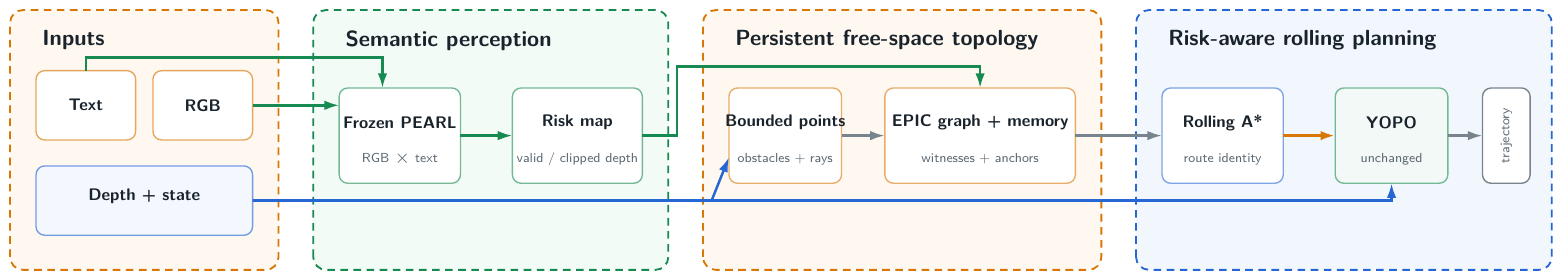
\includegraphics[width=0.98\textwidth]{pics/system_architecture_paper.pdf}
\caption{ScaleNav architecture. Depth builds a bubble graph with
collision-checked edge witnesses. RGB and a text query produce patch scores,
which are projected at a fixed optical depth into persistent semantic nodes.
A measured bubble later promotes an \texttt{Unknown} node to
\texttt{Verified}. Witness risk enters rolling A* and the route gate, which
maintain \texttt{frontier\_goal} and the accepted witness. A 10-m lookahead
on the witness produces \texttt{local\_goal}. Ordered corridor bubbles from
the same witness condition the route-aware YOPO. Semantics changes route
cost. It cannot create or validate an edge.}
\label{fig:architecture}
\end{figure*}

%%%%%%%%%%%%%%%%%%%%%%%%%%%%%%%%%%%%%%%%%%%%%%%%%%%%%%%%%%%%%%%%%%%%%%%%%%%%%%%%
\section{RELATED WORK}
\subsection{Local Reactive Flight}
Depth-based reactive planners trade global consistency for low latency.
RAPPIDS partitions a single depth image into rectangular pyramids and tests
candidate trajectories against them \cite{rappids}.
NanoMap keeps a short history of raw range measurements and answers
uncertainty-aware proximity queries without a global map \cite{nanomap}.
EGO-Planner removes the ESDF from the local optimization loop
\cite{egoplanner}, and learned policies collapse sensing, search, and
optimization into one network pass \cite{yopo,loquercio}.
All of these methods decide motion from what is visible now. None of them
remembers which side of a distant wall was chosen seconds earlier. None of
them accepts semantic intent. ScaleNav therefore keeps such a policy
unchanged as its fast layer and adds memory and semantics around it, not
inside it.

\subsection{Persistent Free-Space Structure}
A second line of work builds structure that outlives one sensor frame.
FUEL maintains frontier information incrementally and plans hierarchically
for fast exploration \cite{fuel}.
FAR Planner updates a global visibility graph as obstacles are observed
\cite{far}, and Bubble Planner extends receding safe corridors for
high-speed flight \cite{bubble}.
EPIC clusters free-space spheres from point clouds into a lightweight
topology for large-scale exploration \cite{epic}.
These structures are purely geometric. Their costs encode distance or
information gain, so a text query such as ``avoid the crowd'' has no
representation. ScaleNav reuses the EPIC-style free-space representation but
solves a different problem. It performs goal-directed rolling search. It
preserves a selected witness route across asynchronous graph replacement.
And it lets edges carry open-vocabulary risk while geometric validity
remains unchanged.

\subsection{Open-Vocabulary Perception and Semantic Navigation}
Open-vocabulary models supply image evidence beyond a fixed label set.
CLIP aligns image and text embeddings \cite{clip}. PEARL produces
training-free open-vocabulary segmentation aligned with image geometry
\cite{pearl}.
On the planning side, VLFM builds vision-language value maps to select
frontiers for object navigation \cite{vlfm}. RayFronts encodes open-set
semantics on mapped voxels and beyond-range rays for online exploration
\cite{rayfronts}.
These systems bring semantics into the map or the frontier score, but the
map itself is the product. How a route should bend around a risky region
before the sensor reaches it is left to a separate decision layer.
ScaleNav targets exactly this interface. Sparse image-space observations
become persistent costs on free-space edges, including observations whose
depth is clipped. Collision validity remains purely geometric.

%%%%%%%%%%%%%%%%%%%%%%%%%%%%%%%%%%%%%%%%%%%%%%%%%%%%%%%%%%%%%%%%%%%%%%%%%%%%%%%%
\section{PROBLEM FORMULATION}
Let the vehicle state at time $t$ be
$\vect{x}_t=(\vect{p}_t,\vect{v}_t,\vect{a}_t,\vect{R}_t)$.
The sensors provide an RGB image $I_t$, a planar-depth image $D_t$, and
odometry.
The mission gives a world-frame goal $\vect{g}$ and a text query $q$ that
describes regions to avoid.
No prior geometric map is available.

The planner must output a dynamically feasible local trajectory $\tau_t$.
We separate this problem into a slow route decision and a fast motion
decision:
\begin{align}
  \vect{g}^{\mathrm{loc}}_t
    &= \Pi_{\mathrm{topo}}(\mathcal{G}_t,I_{0:t},D_{0:t},q,\vect{g}), \\
  \tau_t
    &= \Pi_{\mathrm{local}}(D_t,\vect{v}_t,\vect{a}_t,
       \vect{R}_t^\top(\vect{g}^{\mathrm{loc}}_t-\vect{p}_t)).
\end{align}
In the current system, $\Pi_{\mathrm{local}}$ is the released YOPO runtime.
Its input remains one $160\times96$ depth channel and
\begin{equation}
 \vect{o}_t = [\vect{v}^{B}_t,\vect{a}^{B}_t,
                (\vect{g}^{\mathrm{loc}}_t-\vect{p}_t)^{B}] \in \R^9.
\end{equation}
Only $\Pi_{\mathrm{topo}}$ is introduced by ScaleNav.

We use a fixed-height planning layer in the current experiments to isolate
the horizontal branch-selection problem.
Depth sensing, point memory, and local trajectory execution remain 3-D.
The proposed semantic cost is defined on 3-D witness polylines and does not
require the fixed-height assumption.

%%%%%%%%%%%%%%%%%%%%%%%%%%%%%%%%%%%%%%%%%%%%%%%%%%%%%%%%%%%%%%%%%%%%%%%%%%%%%%%%
\section{PERSISTENT FREE-SPACE TOPOLOGY}
\label{sec:topology}
\subsection{Bounded Geometric Memory}
Depth is back-projected into obstacle points and free-ray evidence.
The implementation voxel-filters this stream and retains at most $N_{\max}$
points within a radius $R_m$ of the vehicle.
It does not construct occupancy voxels or an ESDF.

Following EPIC \cite{epic}, collision-free bubbles are clustered into graph
vertices.
A vertex is
\begin{equation}
 v_i=(\vect{c}_i,\rho_i,z_i,h_i),
\end{equation}
where $\vect{c}_i$ is its center, $\rho_i$ is free-space clearance, $z_i$ is
semantic state, and $h_i$ is a persistent identity record.
An edge stores a collision-checked witness polyline
\begin{equation}
 \pi_{ij}=\{\vect{w}^{ij}_0,\ldots,\vect{w}^{ij}_{M_{ij}}\},
 \quad
 L_{ij}=\sum_{m=1}^{M_{ij}}
 \|\vect{w}^{ij}_m-\vect{w}^{ij}_{m-1}\|_2.
\end{equation}
The witness serves two roles. It is the executable geometric connection. It
is also the support on which semantic distance is measured. The chord
$\vect{c}_j-\vect{c}_i$ is insufficient, because a valid witness may bend
around an obstacle.

Geometry is updated in a background graph. After local bubble generation,
region clustering, and graph connection, an atomic swap exposes the new
graph to planning. The point budget and the spatial radius bound memory.
Transiently missing bubbles receive a short grace period before deletion.

\subsection{Clearance-Aware Edge Cost}
Let $\rho_{ij}=\min(\rho_i,\rho_j)$ and let $\rho^\star$ be the target
clearance.
The implemented soft clearance term is
\begin{equation}
 C_{\mathrm{clr}}(e_{ij})=
 \lambda_{\mathrm{clr}}L_{ij}
 \left[
 \max\left(0,\frac{\rho^\star-\rho_{ij}}{\rho^\star}\right)
 \right]^2.
\label{eq:clearance}
\end{equation}
It prefers open routes but never declares a narrow valid edge invalid.
Geometric feasibility remains determined by the bubble graph and its witness
checks.

%%%%%%%%%%%%%%%%%%%%%%%%%%%%%%%%%%%%%%%%%%%%%%%%%%%%%%%%%%%%%%%%%%%%%%%%%%%%%%%%
\section{SEMANTIC FORESIGHT}
\label{sec:semantics}
\subsection{Semantic Observation Model}
The frozen PEARL model maps $(I_t,q)$ to a patch heatmap.
The heatmap is max-pooled on a $5\times3$ grid. A low-quantile background
baseline is subtracted, so weak whole-image responses do not become risk.
Every retained patch is projected by the calibrated pinhole model at a fixed
optical-axis depth $\ell_s$, independent of the measured depth:
\begin{equation}
 \vect{y}_{u,t}=\vect{p}_t+\mat{R}_t
 \left(\vect{t}_{\mathrm{cam}}+\ell_s\widetilde{\vect{d}}_u\right),
\label{eq:projection}
\end{equation}
where $\vect{p}_t$ and $\mat{R}_t$ are the body pose,
$\vect{t}_{\mathrm{cam}}$ is the camera translation, and
$\widetilde{\vect{d}}_u=[1,x_u,y_u]^\top$ is the unnormalized pinhole ray.
Every endpoint thus has the same optical-axis depth, while off-axis endpoints
have a larger Euclidean range. Measured depth is never consulted by this
projection. It therefore cannot suppress semantic evidence.
For a graph node $v_i$, the associated observation is
\begin{equation}
 \hat{s}_{i,t}=
 \max_{u:\|\vect{y}_{u,t}-\vect{c}_i\|\le r_a}
 s_{u,t}
 \exp\left(-\frac{\|\vect{y}_{u,t}-\vect{c}_i\|^2}{2\sigma_a^2}\right).
\label{eq:association}
\end{equation}
An exponential moving average removes single-frame score jumps:
\begin{equation}
 s_{i,t}=(1-\alpha)s_{i,t-1}+\alpha\hat{s}_{i,t}.
\label{eq:ema}
\end{equation}
The tuple $(s_i,c_i)$ denotes the stored score and confidence. It is restored
by persistent node identity after graph replacement.
Four evidence factors modulate the confidence: multi-row consistency, FOV
margin, suspected ground response, and observation freshness. None of them
rejects an observation outright.

\subsection{Far-Field Semantic Nodes}
Each projected point $\vect{y}_{u,t}$ becomes a persistent graph node with
unknown geometry state and a semantic score.
Repeat observations within $r_m$ update the same node through
(\ref{eq:ema}). Overlapping fields of view across frames re-use the same
persistent identity through ray association.
The node set is bounded by a maximum count, a minimum score, and a minimum
mutual separation. Nodes do not expire with time.
Semantic nodes are stored with the global graph and survive the sliding
geometric window. Risk queries touch only nodes inside the local planning
radius plus an influence band.
Each node is connected through the same local graph machinery as geometric
nodes. When measured geometry later grows a bubble at the node's position,
the node is promoted from unknown to verified while its semantic identity is
retained.

A far-field semantic node is not a hard obstacle. It is a hypothesis about
route risk beyond valid depth. This distinction lets low-risk clipped rays
remain useful as forward graph hypotheses, while high-risk rays repel the
selected route.

\subsection{Continuous Risk on Witness Paths}
Endpoint-only node costs react too late. A risky semantic node may sit
beyond a fork while neither endpoint of the fork carries a high score.
We therefore measure every semantic node against the complete witness
polyline:
\begin{equation}
 d_{k,ij}=\min_{\vect{x}\in\pi_{ij}}
             \|\vect{y}_k-\vect{x}\|_2.
\label{eq:anchor_distance}
\end{equation}
The measured endpoint risk is
\begin{equation}
 r^{\mathrm{node}}_{ij}=\frac{1}{2}(s_i c_i+s_j c_j).
\end{equation}
Semantic node $k$ induces the edge risk
\begin{equation}
 r^{\mathrm{ff}}_{k,ij}=s_kc_k
 \exp\left(-\frac{d_{k,ij}^2}{2\sigma_s^2}\right),
 \qquad d_{k,ij}\le R_s.
\label{eq:field}
\end{equation}
The combined risk uses a maximum rather than a sum:
\begin{equation}
 r_{ij}=\max\left(r^{\mathrm{node}}_{ij},
                  \max_k r^{\mathrm{ff}}_{k,ij}\right).
\label{eq:risk}
\end{equation}
Risk therefore never depends on the arbitrary density of nearby semantic
nodes.
The semantic edge penalty is the barrier
\begin{equation}
 C_{\mathrm{sem}}(e_{ij})=
 \lambda_{\mathrm{sem}}L_{ij}[-\log(1-r_{ij})].
\label{eq:semantic_cost}
\end{equation}
It is nearly linear at low risk and grows sharply near unit risk.
The factor $L_{ij}$ makes exposure accumulate with travel distance.

\begin{figure*}[t]
\centering
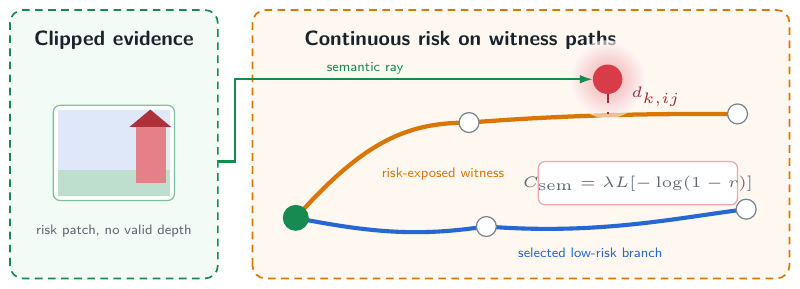
\includegraphics[width=\textwidth]{pics/semantic_risk_field_paper.pdf}
\caption{One logged ScaleNav decision in Map2.
(a)~The logged RGB frame with the PEARL raster and the deployed
$5\!\times\!3$ pooling grid. Numbered rings mark high-response patches whose
synchronized depth has no return.
(b)~The first graph update whose selected witness changes after this
evidence, logged $403$~ms later and drawn top-down in the capture-time body
frame. Matching numbers mark the $30$-m fixed-optical-$Z$ endpoints. Shaded
circles show the $5$-m influence cutoff. Witnesses and nodes are colored by
the confidence-modulated exposure recomputed from the logged endpoints and
witness geometry. Rolling A* selects the teal witness toward
\texttt{frontier\_goal} and away from the exposed branch. Semantics ranks
collision-valid branches. It never changes geometric validity.}
\label{fig:risk_field}
\end{figure*}

%%%%%%%%%%%%%%%%%%%%%%%%%%%%%%%%%%%%%%%%%%%%%%%%%%%%%%%%%%%%%%%%%%%%%%%%%%%%%%%%
\section{RISK-AWARE ROLLING SEARCH}
\subsection{Edge and Path Objectives}
For an edge $e_{ij}$, the geometric traversal cost stored by EPIC is
$W_{ij}$.
Let $\kappa_{ij}=\kappa_{\mathrm{mem}}<1$ if the edge matches the remembered
forward route and $\kappa_{ij}=1$ otherwise.
The complete edge cost is
\begin{equation}
 C(e_{ij})=\kappa_{ij}W_{ij}
          +C_{\mathrm{clr}}(e_{ij})+C_{\mathrm{sem}}(e_{ij}).
\label{eq:edge_cost}
\end{equation}
For a graph path $P$, we accumulate the discounted geometric term and the
risk term separately:
\begin{align}
 G(P)&=\sum_{e\in P}\kappa_eW_e,\\
 R(P)&=\sum_{e\in P}
       \left[C_{\mathrm{clr}}(e)+C_{\mathrm{sem}}(e)\right].
\end{align}
This separation matters. The terminal objective may discount geometry, but
it must never discount safety or semantic exposure.

The slow layer maintains three goal levels: the \emph{mission goal}
$\vect{g}$, a route-level \emph{frontier goal} inside the local graph window
of radius $R_g$, and a control-level \emph{local goal} on the accepted
witness.
The mission goal may lie outside the connected graph. We therefore search
all reachable non-viewpoint vertices within radius $R_g$.
Terminal selection is a single soft loss. Only disconnection, collision,
insufficient clearance, or a missing witness is a hard rejection.
For candidate $v$, let $d_{\mathrm{rsv}}(v)$ be the reserve shortage toward
the mission goal, $d_{\mathrm{dir}}(v)$ the misalignment with the mission
direction, $d_{\mathrm{fov}}(v)$ the offset from the field of view, and
$d_{\mathrm{sm}}(v)$ the heading discontinuity at the vehicle.
The frontier-goal score is
\begin{align}
 J(v)={}&\alpha_gG(P_v)+R(P_v)
       +w_{\mathrm{rsv}}d_{\mathrm{rsv}}(v)+w_{\mathrm{dir}}d_{\mathrm{dir}}(v)
       \nonumber\\
       &+w_{\mathrm{fov}}d_{\mathrm{fov}}(v)
       +w_{\mathrm{sm}}d_{\mathrm{sm}}(v).
\label{eq:terminal}
\end{align}
Direction, FOV, and reserve terms guide the search. They never disqualify a
feasible terminal. Once the mission goal enters the local window, a bubble
search validates the final connection within a short range.
Graph A* uses $f=g+h$ with millisecond-scale connection budgets.
The best recovered path ends at
\begin{equation}
 v_t^\star=\arg\min_{v\in\mathcal{V}_{\mathrm{cand}}}J(v),
\end{equation}
and its terminal becomes the frontier goal.

\subsection{Route Identity Across Graph Updates}
Incremental graph replacement can change node objects even when the physical
route is unchanged.
ScaleNav therefore stores the selected witness in world coordinates:
\begin{equation}
 \mathcal{W}_{t-1}=\{\vect{w}_0,\ldots,\vect{w}_K\}.
\end{equation}
The vehicle is projected onto this polyline, and only a forward window of
length $H_r$ is retained:
\begin{equation}
 \mathcal{W}^{+}_{t-1}=
 \operatorname{crop}(\mathcal{W}_{t-1},
                     \operatorname{proj}(\vect{p}_t,\mathcal{W}_{t-1}),H_r).
\end{equation}
An edge in the new graph is remembered if its geometry follows this window
within a lateral tolerance.
The incumbent terminal is restored by persistent node identity first, with
nearest-neighbor remapping as a fallback.
Equation (\ref{eq:edge_cost}) then provides a soft prior rather than a hard
lock.

A challenger replaces the incumbent only through hysteresis. Its risk must
improve by more than a margin, or its total cost must drop below a fixed
ratio of the incumbent cost.
A high-risk incumbent is latched until its route risk falls back below a
release threshold. Prefix-preserving route extensions are exempt from the
switch test.
The prior is released when the vehicle leaves the route or when semantic
risk along the route changes by more than $\Delta_r$:
\begin{equation}
 \left|\mathcal{R}(\mathcal{W}_{t-1};t)-
        \mathcal{R}(\mathcal{W}_{t-1};t-1)\right|>\Delta_r.
\end{equation}
This balance is central to the design. Route memory prevents left-right
oscillation. Risk-triggered release lets new language evidence change the
homotopy.

\subsection{Route-Conditioned Local Policy}
The graph publishes the accepted witness. A 10-m lookahead on that witness
produces the local goal $\vect{g}^{\mathrm{loc}}_t$.
The same witness is further processed into an ordered corridor of safe
bubbles that conditions the local policy.

The accepted witness is first refined toward a clearance-centered corridor.
Vertices are adjusted with fixed endpoints and protected turning points. A
move is accepted only if every witness segment remains continuously safe and
the bottleneck clearance improves.
From the refined witness we sample ordered corridor bubbles
\begin{equation}
 b_k=(\vect{c}_k,r_k),\quad
 r_k=\max\left(0,d(\vect{c}_k)-r_{\mathrm{rob}}-r_{\mathrm{safe}}\right),
\label{eq:bubble}
\end{equation}
where $d(\vect{c}_k)$ is the obstacle distance at center $\vect{c}_k$.
YOPO receives depth, body velocity and acceleration, the frontier goal, and
a fixed-$K$ ordered bubble list with a route mask:
\begin{equation}
 \mathcal{B}_t=\{([\vect{c}_k^{B}]_t,r_k)\}_{k=1}^{K}.
\label{eq:route_input}
\end{equation}
The network still predicts primitive terminal states and scores. The
trajectory generator is unchanged.
The score cost adds a route term that prefers staying inside the selected
corridor, progressing along its arc length, and aligning with the local
witness tangent:
\begin{equation}
 L_{\mathrm{cor}}=\frac{1}{N}\sum_{n=1}^{N}
 \min_k\max\left(0,\|\vect{p}_n-\vect{c}_k\|_2-r_k\right)^2.
\label{eq:corridor_loss}
\end{equation}
There is no behavior cloning. The witness is a geometric corridor, not a
timed expert trajectory.
This gives a clean division of labor: the graph chooses which corridor to
follow, and YOPO decides the exact trajectory inside it.

%%%%%%%%%%%%%%%%%%%%%%%%%%%%%%%%%%%%%%%%%%%%%%%%%%%%%%%%%%%%%%%%%%%%%%%%%%%%%%%%
\section{EXPERIMENTS AND RESULTS}
\label{sec:experiments}

\subsection{Experimental Setup}
We evaluate ScaleNav in Colosseum/AirSim \cite{airsim} with synchronized
RGB-D and odometry. The current evaluation uses a 1.6-m horizontal graph
layer.
Each condition runs at least 20 paired trials with identical starts, goals,
scenes, and random seeds across methods.
We report mean, standard deviation, and a 95\% confidence interval. Paired
continuous metrics use a two-sided Wilcoxon signed-rank test. Success
proportions use paired bootstrap intervals. Failed trials remain in the
safety and success metrics and are never removed from path-efficiency
statistics.
All ScaleNav variants share graph and local-policy parameters.
Table~\ref{tab:params} lists the main runtime settings.

\begin{table}[t]
\caption{Fixed Parameters Used by the Current Implementation}
\label{tab:params}
\centering
\small
\resizebox{\columnwidth}{!}{%
\begin{tabular}{lc@{\quad}lc}
\toprule
Parameter & Value & Parameter & Value \\
\midrule
Point voxel & 0.10 m & Point budget & 100,000 \\
Memory radius & 40 m & Graph update & 100 ms \\
Graph rebuild & 100 ms & Search radius & 35 m \\
Local lookahead & 10 m & Goal-connect budget & 20 ms \\
$\lambda_{\rm sem}$ & 2.0 & $R_s$ & 10 m \\
$\lambda_{\rm clr}$ & 2.0 & $\rho^\star$ & 1.2 m \\
$\alpha$ in (\ref{eq:ema}) & 0.3 & $\kappa_{\rm mem}$ & 0.9 \\
Optical depth $\ell_s$ & 30 m & Node merge distance & 2.5 m \\
Maximum semantic nodes & 16 & Semantic grid & $5\times3$ \\
\bottomrule
\end{tabular}
}
\end{table}

\subsection{Overall Navigation Performance}
The benchmark contains six paired scenario families: long-detour walls;
semantic forks beyond clipped depth; late-arriving semantic contradictions;
mixed-scale flights with detours and narrow passages; corridor conflicts
that test route memory against blind following; and compositional-language
queries with hard negatives. Scene complexity is varied by obstacle density,
free-space width, detour length, and the number of competing branches.

We compare the following methods:
\begin{itemize}
  \item \textbf{YOPO}: the original local planner with the mission goal.
  \item \textbf{EGO-Planner}: a representative ESDF-free geometric local
  planner \cite{egoplanner}.
  \item \textbf{FAR Planner}: a visibility-graph baseline \cite{far}, using
  the same sensor range and local executor where the implementation permits.
  \item \textbf{Geometry}: the persistent EPIC graph and rolling goal with
  all semantic weights set to zero.
  \item \textbf{ScaleNav}: the full system with semantic foresight and route
  conditioning.
\end{itemize}

Success requires reaching the goal without collision or timeout. Path and
time statistics include failed trials, so methods that terminate early gain
no advantage.
Table~\ref{tab:main_results} reports closed-loop navigation performance
across all scenario families. A dash denotes an unreported measurement, not
a zero: entries are filled only after all paired trials of a condition pass
the same logging and validation protocol.

\begin{table*}[t]
\caption{Closed-Loop Navigation Performance}
\label{tab:main_results}
\centering
\small
\resizebox{\textwidth}{!}{%
\begin{tabular}{lcccccccc}
\toprule
Method & Success (\%) & Collision (\%) & $L$ (m) & $T$ (s) &
$\bar v$ (m/s) & $d_{\min}$ (m) & $\bar d_{\rm obs}$ (m) & $E_{\rm sem}$ \\
\midrule
YOPO             & \blank & \blank & \blank & \blank & \blank & \blank & \blank & \blank \\
EGO-Planner      & \blank & \blank & \blank & \blank & \blank & \blank & \blank & \blank \\
FAR Planner      & \blank & \blank & \blank & \blank & \blank & \blank & \blank & \blank \\
Geometry         & \blank & \blank & \blank & \blank & \blank & \blank & \blank & \blank \\
ScaleNav (ours)  & \blank & \blank & \blank & \blank & \blank & \blank & \blank & \blank \\
\bottomrule
\end{tabular}
}
\end{table*}

We report path length, average speed, minimum and average obstacle distance,
semantic exposure $E_{\mathrm{sem}}=\frac{1}{L}\int_0^T r(\vect{p}(t))v(t)\,dt$,
route-switch count, success, collision, completion time, and semantic task
compliance.
For semantic forks we additionally measure the decision distance at which
the selected route commits to the correct branch.

\subsection{Semantic Foresight and Route Stability}
The semantic-fork and contradiction scenarios isolate early branch selection
from geometric collision avoidance.
The component study uses five ablations. \emph{Measured} adds semantic
memory only on depth-verified nodes. \emph{Endpoint} additionally retains
far-field nodes but applies their cost only at edge endpoints. \emph{Field}
uses the continuous witness-field cost. \emph{Field-NoMem} disables the
route-memory discount. \emph{Field-NoRelease} disables risk-triggered route
release.
Table~\ref{tab:semantic_results} separates these factors.

\begin{table}[t]
\caption{Semantic Foresight and Route-Stability Ablations}
\label{tab:semantic_results}
\centering
\small
\resizebox{\columnwidth}{!}{%
\begin{tabular}{lcccc}
\toprule
Method & Correct branch & Decision dist. & Switches & $E_{\rm sem}$ \\
       & (\%) & (m) & (count) & \\
\midrule
Measured        & \blank & \blank & \blank & \blank \\
Endpoint        & \blank & \blank & \blank & \blank \\
Field (ours)    & \blank & \blank & \blank & \blank \\
Field-NoMem     & \blank & \blank & \blank & \blank \\
Field-NoRelease & \blank & \blank & \blank & \blank \\
\bottomrule
\end{tabular}
}
\end{table}

\subsection{Route-Conditioned YOPO}
Table~\ref{tab:yopo_results} compares route conditioning against waypoint
conditioning under identical depth, motion, and frontier-goal inputs.
Route-YOPO halves the corridor-violation rate, from $61.50\%$ to $30.00\%$,
and reduces the collision rate from $20.33\%$ to $17.33\%$.

The model is trained on $3{,}000$ pilot routes with the corridor
representation and the route-conditioned loss in (\ref{eq:corridor_loss}).
The pilot set contains $53.53\%$ forced detours and a continuous minimum
clearance of $0.544$~m.
Validation on $300$ held-out routes shows zero collisions and $0.745$~m
minimum clearance.
The independent $1{,}200$-route test set shows zero collisions, $0.623$~m
minimum clearance, $0.0090$~m average maximum bubble-union violation, and
$5.348$~m average route progress.

\begin{table}[t]
\caption{Route Conditioning on the Real-Tree Benchmark}
\label{tab:yopo_results}
\centering
\small
\begin{tabular}{lccc}
\toprule
Method & Success (\%) & Collision (\%) & Corr. viol. (\%) \\
\midrule
YOPO-Simple & \blank & 20.33 & 61.50 \\
Route-YOPO  & \textbf{82.67} & \textbf{17.33} & \textbf{30.00} \\
\bottomrule
\end{tabular}
\end{table}

\subsection{Runtime and Resource Usage}
Table~\ref{tab:runtime_results} decomposes the end-to-end compute cost.
Latency is reported as the mean and 99th percentile. Rate and memory are
measured during the same closed-loop runs.
System metrics are PEARL latency, graph-update wall time, A* latency, graph
size, resident memory, local-policy rate, and dropped semantic frames.

\begin{table}[t]
\caption{Runtime and Memory Cost}
\label{tab:runtime_results}
\centering
\small
\resizebox{\columnwidth}{!}{%
\begin{tabular}{lcccc}
\toprule
Module & Mean (ms) & P99 (ms) & Rate (Hz) & Memory (MB) \\
\midrule
PEARL inference & \blank & \blank & \blank & \blank \\
Graph update    & \blank & \blank & \blank & \blank \\
Rolling A*      & \blank & \blank & \blank & \blank \\
YOPO inference  & \blank & \blank & \blank & \blank \\
Full system     & \blank & \blank & \blank & \blank \\
\bottomrule
\end{tabular}
}
\end{table}

\FloatBarrier

%%%%%%%%%%%%%%%%%%%%%%%%%%%%%%%%%%%%%%%%%%%%%%%%%%%%%%%%%%%%%%%%%%%%%%%%%%%%%%%%
\section{DISCUSSION AND LIMITATIONS}
ScaleNav adds route-scale memory and semantic branch guidance to an existing
local planner. It does not replace the planner's dynamic-obstacle response,
and it never turns semantics into a safety certificate.
Far-field semantic nodes are deliberately optimistic geometry. A false
positive causes a longer route. A false negative falls back to geometric
topology and local depth avoidance.
The bounded Gaussian field, the bounded node set, EMA updates, and the
confidence factors limit both spatial and temporal error growth.

The current experiments restrict topological search to a fixed-height layer.
This isolates the left-right detour problem but does not evaluate vertical
homotopy choices. Evaluating the same witness-field cost on a fully 3-D
graph is future work.
The semantic front end follows a model-independent observation contract. A
larger vision-language model can therefore replace PEARL without changing
the projection, EMA, or edge-risk equations, and without changing the
planner's safety contract.

%%%%%%%%%%%%%%%%%%%%%%%%%%%%%%%%%%%%%%%%%%%%%%%%%%%%%%%%%%%%%%%%%%%%%%%%%%%%%%%%
\section{CONCLUSION}
This paper presented ScaleNav, a vision-based aerial navigation system that
adds semantic foresight at the topological route layer.
Depth-clipped open-vocabulary observations become persistent far-field
semantic nodes. Their continuous risk field acts on collision-checked
witness paths and can change a branch before the risk is geometrically
observed.
A world-frame witness memory preserves route identity across asynchronous
graph replacement. A route-conditioned YOPO variant flies inside the
selected corridor.
The result is a clean separation of concerns: topology remembers, semantics
ranks, and the local policy flies.

%%%%%%%%%%%%%%%%%%%%%%%%%%%%%%%%%%%%%%%%%%%%%%%%%%%%%%%%%%%%%%%%%%%%%%%%%%%%%%%%
{\footnotesize
\begin{thebibliography}{99}
\bibitem{yopo}
J. Lu, X. Zhang, H. Shen, L. Xu, and B. Tian,
``You Only Plan Once: A Learning-Based One-Stage Planner With Guidance Learning,''
\emph{IEEE Robotics and Automation Letters}, vol. 9, no. 7,
pp. 6083--6090, 2024.

\bibitem{rappids}
N. Bucki, J. Lee, and M. W. Mueller,
``Rectangular Pyramid Partitioning Using Integrated Depth Sensors (RAPPIDS): A Fast Planner for Multicopter Navigation,''
\emph{IEEE Robotics and Automation Letters}, vol. 5, no. 3,
pp. 4626--4633, 2020.

\bibitem{nanomap}
P. R. Florence, J. Carter, J. Ware, and R. Tedrake,
``NanoMap: Fast, Uncertainty-Aware Proximity Queries With Lazy Search of Local 3-D Data,''
in \emph{Proc. IEEE Int. Conf. Robot. Autom.}, 2018, pp. 7631--7638.

\bibitem{egoplanner}
X. Zhou, Z. Wang, H. Ye, C. Xu, and F. Gao,
``EGO-Planner: An ESDF-Free Gradient-Based Local Planner for Quadrotors,''
\emph{IEEE Robotics and Automation Letters}, vol. 6, no. 2,
pp. 478--485, 2021.

\bibitem{loquercio}
A. Loquercio, E. Kaufmann, R. Ranftl, M. M\"uller, V. Koltun, and D. Scaramuzza,
``Learning High-Speed Flight in the Wild,''
\emph{Science Robotics}, vol. 6, no. 59, 2021.

\bibitem{fuel}
B. Zhou, Y. Zhang, X. Chen, and S. Shen,
``FUEL: Fast UAV Exploration Using Incremental Frontier Structure and Hierarchical Planning,''
\emph{IEEE Robotics and Automation Letters}, vol. 6, no. 2,
pp. 779--786, 2021.

\bibitem{far}
F. Yang, C. Cao, H. Zhu, J. Oh, and J. Zhang,
``FAR Planner: Fast, Attemptable Route Planner Using Dynamic Visibility Update,''
in \emph{Proc. IEEE/RSJ Int. Conf. Intell. Robots Syst.}, 2022, pp. 9--16.

\bibitem{bubble}
Y. Ren, F. Zhu, W. Liu, Z. Wang, Y. Lin, F. Gao, and F. Zhang,
``Bubble Planner: Planning High-Speed Smooth Quadrotor Trajectories Using Receding Corridors,''
in \emph{Proc. IEEE/RSJ Int. Conf. Intell. Robots Syst.}, 2022,
pp. 6332--6339.

\bibitem{epic}
S. Geng, Z. Ning, F. Zhang, and B. Zhou,
``EPIC: A Lightweight LiDAR-Based AAV Exploration Framework for Large-Scale Scenarios,''
\emph{IEEE Robotics and Automation Letters}, vol. 10, no. 5,
pp. 5090--5097, 2025.

\bibitem{clip}
A. Radford et al.,
``Learning Transferable Visual Models From Natural Language Supervision,''
in \emph{Proc. Int. Conf. Mach. Learn.}, 2021, pp. 8748--8763.

\bibitem{pearl}
G. Pei, X. Jiang, X. Cai, T. Chen, Y. Yao, and B. Jeon,
``PEARL: Geometry Aligns Semantics for Training-Free Open-Vocabulary Semantic Segmentation,''
\emph{arXiv preprint arXiv:2603.21528}, 2026.

\bibitem{vlfm}
N. Yokoyama, S. Ha, D. Batra, J. Wang, and B. Bucher,
``VLFM: Vision-Language Frontier Maps for Zero-Shot Semantic Navigation,''
in \emph{Proc. IEEE Int. Conf. Robot. Autom.}, 2024, pp. 42--48.

\bibitem{rayfronts}
O. Alama, A. Bhattacharya, H. He, S. Kim, Y. Qiu, W. Wang, C. Ho, N. Keetha, and S. Scherer,
``RayFronts: Open-Set Semantic Ray Frontiers for Online Scene Understanding and Exploration,''
in \emph{Proc. IEEE/RSJ Int. Conf. Intell. Robots Syst.}, 2025, pp. 5930--5937.

\bibitem{airsim}
S. Shah, D. Dey, C. Lovett, and A. Kapoor,
``AirSim: High-Fidelity Visual and Physical Simulation for Autonomous Vehicles,''
in \emph{Field and Service Robotics}, 2018, pp. 621--635.
\end{thebibliography}
}

\end{document}
